\documentclass[twoside]{book}

% Packages required by doxygen
\usepackage{fixltx2e}
\usepackage{calc}
\usepackage{doxygen}
\usepackage[export]{adjustbox} % also loads graphicx
\usepackage{graphicx}
\usepackage[utf8]{inputenc}
\usepackage{makeidx}
\usepackage{multicol}
\usepackage{multirow}
\PassOptionsToPackage{warn}{textcomp}
\usepackage{textcomp}
\usepackage[nointegrals]{wasysym}
\usepackage[table]{xcolor}

% NLS support packages
\usepackage[T2A]{fontenc}
\usepackage[russian]{babel}

% Font selection
\usepackage[T1]{fontenc}
\usepackage[scaled=.90]{helvet}
\usepackage{courier}
\usepackage{amssymb}
\usepackage{sectsty}
\renewcommand{\familydefault}{\sfdefault}
\allsectionsfont{%
  \fontseries{bc}\selectfont%
  \color{darkgray}%
}
\renewcommand{\DoxyLabelFont}{%
  \fontseries{bc}\selectfont%
  \color{darkgray}%
}
\newcommand{\+}{\discretionary{\mbox{\scriptsize$\hookleftarrow$}}{}{}}

% Page & text layout
\usepackage{geometry}
\geometry{%
  a4paper,%
  top=2.5cm,%
  bottom=2.5cm,%
  left=2.5cm,%
  right=2.5cm%
}
\tolerance=750
\hfuzz=15pt
\hbadness=750
\setlength{\emergencystretch}{15pt}
\setlength{\parindent}{0cm}
\setlength{\parskip}{0.2cm}
\makeatletter
\renewcommand{\paragraph}{%
  \@startsection{paragraph}{4}{0ex}{-1.0ex}{1.0ex}{%
    \normalfont\normalsize\bfseries\SS@parafont%
  }%
}
\renewcommand{\subparagraph}{%
  \@startsection{subparagraph}{5}{0ex}{-1.0ex}{1.0ex}{%
    \normalfont\normalsize\bfseries\SS@subparafont%
  }%
}
\makeatother

% Headers & footers
\usepackage{fancyhdr}
\pagestyle{fancyplain}
\fancyhead[LE]{\fancyplain{}{\bfseries\thepage}}
\fancyhead[CE]{\fancyplain{}{}}
\fancyhead[RE]{\fancyplain{}{\bfseries\leftmark}}
\fancyhead[LO]{\fancyplain{}{\bfseries\rightmark}}
\fancyhead[CO]{\fancyplain{}{}}
\fancyhead[RO]{\fancyplain{}{\bfseries\thepage}}
\fancyfoot[LE]{\fancyplain{}{}}
\fancyfoot[CE]{\fancyplain{}{}}
\fancyfoot[RE]{\fancyplain{}{\bfseries\scriptsize Документация по T\+R\+P\+O. Последние изменения\+: Пт 3 Июн 2016 19\+:43\+:24. Создано системой Doxygen }}
\fancyfoot[LO]{\fancyplain{}{\bfseries\scriptsize Документация по T\+R\+P\+O. Последние изменения\+: Пт 3 Июн 2016 19\+:43\+:24. Создано системой Doxygen }}
\fancyfoot[CO]{\fancyplain{}{}}
\fancyfoot[RO]{\fancyplain{}{}}
\renewcommand{\footrulewidth}{0.4pt}
\renewcommand{\chaptermark}[1]{%
  \markboth{#1}{}%
}
\renewcommand{\sectionmark}[1]{%
  \markright{\thesection\ #1}%
}

% Indices & bibliography
\usepackage{natbib}
\usepackage[titles]{tocloft}
\setcounter{tocdepth}{3}
\setcounter{secnumdepth}{5}
\makeindex

% Hyperlinks (required, but should be loaded last)
\usepackage{ifpdf}
\ifpdf
  \usepackage[pdftex,pagebackref=true]{hyperref}
\else
  \usepackage[ps2pdf,pagebackref=true]{hyperref}
\fi
\hypersetup{%
  colorlinks=true,%
  linkcolor=blue,%
  citecolor=blue,%
  unicode%
}

% Custom commands
\newcommand{\clearemptydoublepage}{%
  \newpage{\pagestyle{empty}\cleardoublepage}%
}


%===== C O N T E N T S =====

\begin{document}

% Titlepage & ToC
\hypersetup{pageanchor=false,
             bookmarks=true,
             bookmarksnumbered=true,
             pdfencoding=unicode
            }
\pagenumbering{roman}
\begin{titlepage}
\vspace*{7cm}
\begin{center}%
{\Large T\+R\+P\+O }\\
\vspace*{1cm}
{\large Создано системой Doxygen 1.8.9.1}\\
\vspace*{0.5cm}
{\small Пт 3 Июн 2016 19:43:24}\\
\end{center}
\end{titlepage}
\clearemptydoublepage
\tableofcontents
\clearemptydoublepage
\pagenumbering{arabic}
\hypersetup{pageanchor=true}

%--- Begin generated contents ---
\chapter{trpo-\/dz}
\label{md_README}
\hypertarget{md_README}{}
ДЗ ТРПО

\subsection*{Diagrams}

\subsubsection*{class diagram of the backend}



\subsubsection*{object diagram of the frontend}

 
\chapter{Иерархический список классов}
\section{Иерархия классов}
Иерархия классов.\begin{DoxyCompactList}
\item \contentsline{section}{Basic\+Gateway}{\pageref{classBasicGateway}}{}
\item \contentsline{section}{Layer\+Communication}{\pageref{classLayerCommunication}}{}
\item \contentsline{section}{Mapper}{\pageref{classMapper}}{}
\begin{DoxyCompactList}
\item \contentsline{section}{Discipline\+Mapper}{\pageref{classDisciplineMapper}}{}
\item \contentsline{section}{Materials\+Mapper}{\pageref{classMaterialsMapper}}{}
\end{DoxyCompactList}
\item \contentsline{section}{Moget\+Otvetchat}{\pageref{interfaceMogetOtvetchat}}{}
\begin{DoxyCompactList}
\item \contentsline{section}{Model}{\pageref{classModel}}{}
\begin{DoxyCompactList}
\item \contentsline{section}{Basic\+Model}{\pageref{classBasicModel}}{}
\begin{DoxyCompactList}
\item \contentsline{section}{Disciplines\+Model}{\pageref{classDisciplinesModel}}{}
\item \contentsline{section}{Materials\+Model}{\pageref{classMaterialsModel}}{}
\item \contentsline{section}{Professors\+Model}{\pageref{classProfessorsModel}}{}
\end{DoxyCompactList}
\item \contentsline{section}{Student\+Adapter}{\pageref{classStudentAdapter}}{}
\end{DoxyCompactList}
\end{DoxyCompactList}
\item P\+D\+O\begin{DoxyCompactList}
\item \contentsline{section}{Database}{\pageref{classDatabase}}{}
\end{DoxyCompactList}
\item \contentsline{section}{Table\+Module}{\pageref{classTableModule}}{}
\begin{DoxyCompactList}
\item \contentsline{section}{Disciplines}{\pageref{classDisciplines}}{}
\item \contentsline{section}{Materials}{\pageref{classMaterials}}{}
\end{DoxyCompactList}
\end{DoxyCompactList}

\chapter{Алфавитный указатель классов}
\section{Классы}
Классы с их кратким описанием.\begin{DoxyCompactList}
\item\contentsline{section}{\hyperlink{classBasicGateway}{Basic\+Gateway} }{\pageref{classBasicGateway}}{}
\item\contentsline{section}{\hyperlink{classBasicModel}{Basic\+Model} }{\pageref{classBasicModel}}{}
\item\contentsline{section}{\hyperlink{classDatabase}{Database} }{\pageref{classDatabase}}{}
\item\contentsline{section}{\hyperlink{classDisciplineMapper}{Discipline\+Mapper} }{\pageref{classDisciplineMapper}}{}
\item\contentsline{section}{\hyperlink{classDisciplines}{Disciplines} }{\pageref{classDisciplines}}{}
\item\contentsline{section}{\hyperlink{classDisciplinesModel}{Disciplines\+Model} }{\pageref{classDisciplinesModel}}{}
\item\contentsline{section}{\hyperlink{classLayerCommunication}{Layer\+Communication} }{\pageref{classLayerCommunication}}{}
\item\contentsline{section}{\hyperlink{classMapper}{Mapper} }{\pageref{classMapper}}{}
\item\contentsline{section}{\hyperlink{classMaterials}{Materials} }{\pageref{classMaterials}}{}
\item\contentsline{section}{\hyperlink{classMaterialsMapper}{Materials\+Mapper} }{\pageref{classMaterialsMapper}}{}
\item\contentsline{section}{\hyperlink{classMaterialsModel}{Materials\+Model} }{\pageref{classMaterialsModel}}{}
\item\contentsline{section}{\hyperlink{classModel}{Model} }{\pageref{classModel}}{}
\item\contentsline{section}{\hyperlink{interfaceMogetOtvetchat}{Moget\+Otvetchat} }{\pageref{interfaceMogetOtvetchat}}{}
\item\contentsline{section}{\hyperlink{classProfessorsModel}{Professors\+Model} }{\pageref{classProfessorsModel}}{}
\item\contentsline{section}{\hyperlink{classStudentAdapter}{Student\+Adapter} }{\pageref{classStudentAdapter}}{}
\item\contentsline{section}{\hyperlink{classTableModule}{Table\+Module} }{\pageref{classTableModule}}{}
\end{DoxyCompactList}

\chapter{Классы}
\hypertarget{classBasicGateway}{}\section{Класс Basic\+Gateway}
\label{classBasicGateway}\index{Basic\+Gateway@{Basic\+Gateway}}
\subsection*{Открытые члены}
\begin{DoxyCompactItemize}
\item 
\hypertarget{classBasicGateway_a8f81fcf05bbf2ecccf1c8ac68043e58f}{}\hyperlink{classBasicGateway_a8f81fcf05bbf2ecccf1c8ac68043e58f}{\+\_\+\+\_\+construct} (\hyperlink{classDatabase}{Database} \$db, \$tablename)\label{classBasicGateway_a8f81fcf05bbf2ecccf1c8ac68043e58f}

\begin{DoxyCompactList}\small\item\em Create a new gateway for the given table. \end{DoxyCompactList}\item 
\hypertarget{classBasicGateway_a479340638f40df0f02d833b8326b26d5}{}\hyperlink{classBasicGateway_a479340638f40df0f02d833b8326b26d5}{get\+All} ()\label{classBasicGateway_a479340638f40df0f02d833b8326b26d5}

\begin{DoxyCompactList}\small\item\em Get an array of all elements in the table. \end{DoxyCompactList}\item 
\hyperlink{classBasicGateway_aaca2505381d589b069c4a5ba870be63d}{update} (\$data, \$col, \$val)
\item 
\hyperlink{classBasicGateway_a26ff35b0c74ca7faf3f2aa20cfa8bf18}{create} ()
\item 
\hyperlink{classBasicGateway_ae3acd2ba4018730745410b9cd59aff75}{delete} (\$data)
\end{DoxyCompactItemize}


\subsection{Подробное описание}
Represent a gateway to a database table. This should be used so that business logic classes didn\textquotesingle{}t have to interact with the database 

\subsection{Методы}
\hypertarget{classBasicGateway_a26ff35b0c74ca7faf3f2aa20cfa8bf18}{}\index{Basic\+Gateway@{Basic\+Gateway}!create@{create}}
\index{create@{create}!Basic\+Gateway@{Basic\+Gateway}}
\subsubsection[{create}]{\setlength{\rightskip}{0pt plus 5cm}Basic\+Gateway\+::create (
\begin{DoxyParamCaption}
{}
\end{DoxyParamCaption}
)}\label{classBasicGateway_a26ff35b0c74ca7faf3f2aa20cfa8bf18}
Add an empty element in the table \hypertarget{classBasicGateway_ae3acd2ba4018730745410b9cd59aff75}{}\index{Basic\+Gateway@{Basic\+Gateway}!delete@{delete}}
\index{delete@{delete}!Basic\+Gateway@{Basic\+Gateway}}
\subsubsection[{delete}]{\setlength{\rightskip}{0pt plus 5cm}Basic\+Gateway\+::delete (
\begin{DoxyParamCaption}
\item[{}]{\$data}
\end{DoxyParamCaption}
)}\label{classBasicGateway_ae3acd2ba4018730745410b9cd59aff75}
Remove an element from the table 
\begin{DoxyParams}{Аргументы}
{\em data} & array \+: The line to remove \\
\hline
\end{DoxyParams}
\hypertarget{classBasicGateway_aaca2505381d589b069c4a5ba870be63d}{}\index{Basic\+Gateway@{Basic\+Gateway}!update@{update}}
\index{update@{update}!Basic\+Gateway@{Basic\+Gateway}}
\subsubsection[{update}]{\setlength{\rightskip}{0pt plus 5cm}Basic\+Gateway\+::update (
\begin{DoxyParamCaption}
\item[{}]{\$data, }
\item[{}]{\$col, }
\item[{}]{\$val}
\end{DoxyParamCaption}
)}\label{classBasicGateway_aaca2505381d589b069c4a5ba870be63d}
Update a given line in the table 
\begin{DoxyParams}{Аргументы}
{\em data} & The current line \\
\hline
{\em col} & Name of the column to update \\
\hline
{\em val} & New value to insert \\
\hline
\end{DoxyParams}

\begin{DoxyExceptions}{Исключения}
{\em Exception} & S\+Q\+L error \\
\hline
\end{DoxyExceptions}
\begin{DoxyReturn}{Возвращает}
An array containing information about the database query (number of affected rows) 
\end{DoxyReturn}


Объявления и описания членов класса находятся в файле\+:\begin{DoxyCompactItemize}
\item 
backend/Basic\+Gateway.\+php\end{DoxyCompactItemize}

\hypertarget{classBasicModel}{}\section{Класс Basic\+Model}
\label{classBasicModel}\index{Basic\+Model@{Basic\+Model}}
Граф наследования\+:Basic\+Model\+:\begin{figure}[H]
\begin{center}
\leavevmode
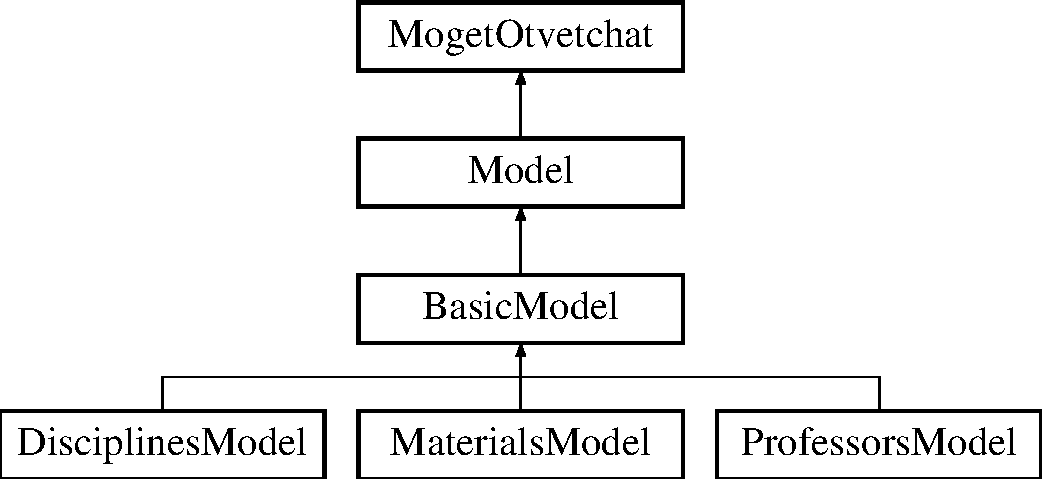
\includegraphics[height=4.000000cm]{classBasicModel}
\end{center}
\end{figure}
\subsection*{Открытые члены}
\begin{DoxyCompactItemize}
\item 
\hypertarget{classBasicModel_a2adeecd61c4fdc6284e879d2a195d550}{}{\bfseries \+\_\+\+\_\+construct} (\hyperlink{classDatabase}{Database} \$db, \$tablename)\label{classBasicModel_a2adeecd61c4fdc6284e879d2a195d550}

\item 
\hypertarget{classBasicModel_a27380f937aa402305546d7624d04efb3}{}{\bfseries get\+Value} (array \$query)\label{classBasicModel_a27380f937aa402305546d7624d04efb3}

\end{DoxyCompactItemize}


Объявления и описания членов класса находятся в файле\+:\begin{DoxyCompactItemize}
\item 
backend/Basic\+Model.\+php\end{DoxyCompactItemize}

\hypertarget{classDatabase}{}\section{Класс Database}
\label{classDatabase}\index{Database@{Database}}
Граф наследования\+:Database\+:\begin{figure}[H]
\begin{center}
\leavevmode
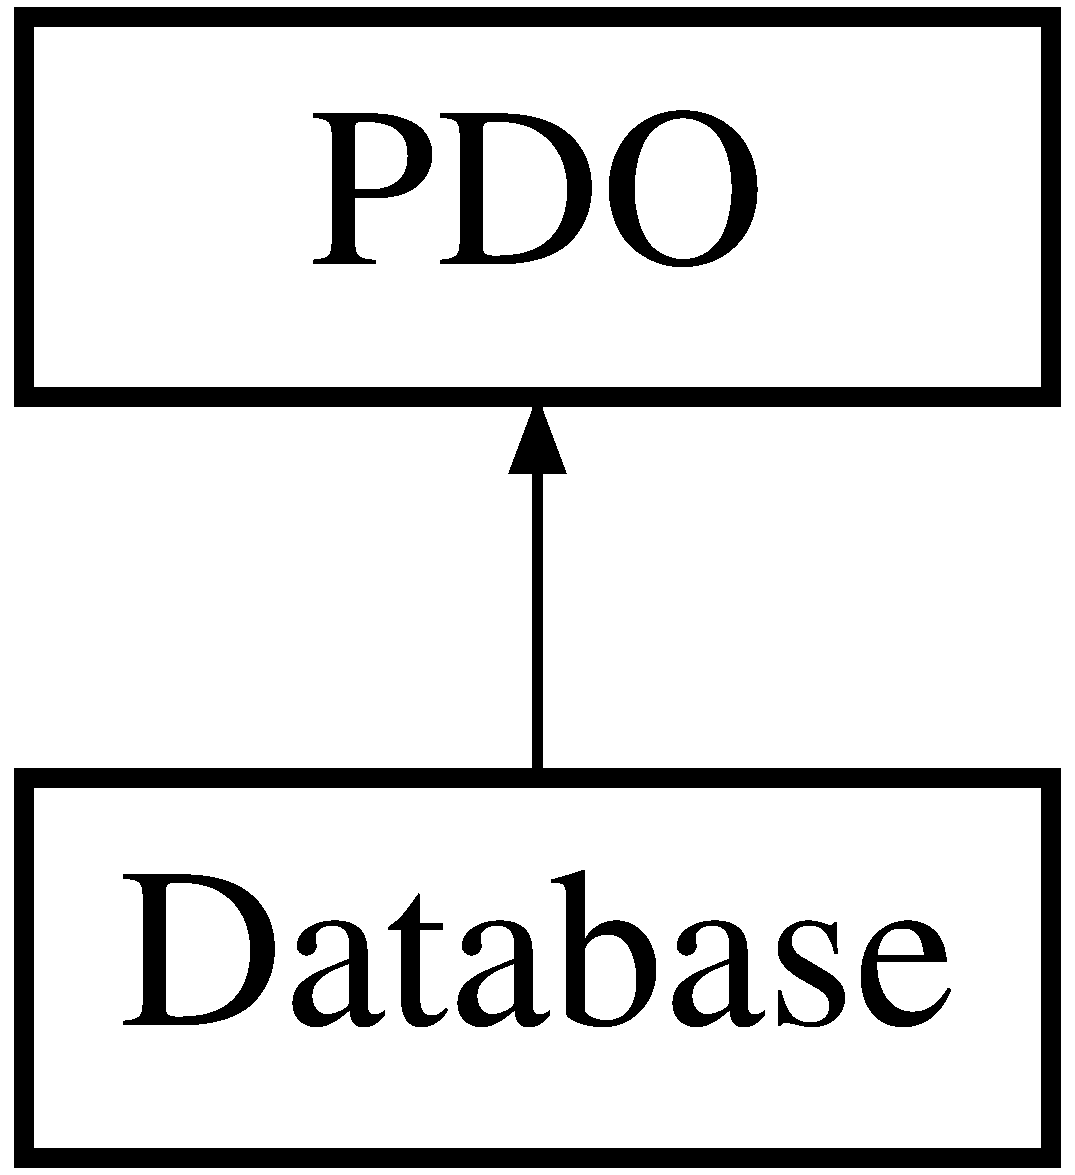
\includegraphics[height=2.000000cm]{classDatabase}
\end{center}
\end{figure}
\subsection*{Открытые члены}
\begin{DoxyCompactItemize}
\item 
\hypertarget{classDatabase_ab2bc6b3afffba0473e1f9026a2af99fb}{}{\bfseries \+\_\+\+\_\+construct} (\$host=N\+U\+L\+L, \$dbname=N\+U\+L\+L, \$username=N\+U\+L\+L, \$passwd=N\+U\+L\+L)\label{classDatabase_ab2bc6b3afffba0473e1f9026a2af99fb}

\end{DoxyCompactItemize}


Объявления и описания членов класса находятся в файле\+:\begin{DoxyCompactItemize}
\item 
backend/Database.\+php\end{DoxyCompactItemize}

\hypertarget{classDisciplineMapper}{}\section{Класс Discipline\+Mapper}
\label{classDisciplineMapper}\index{Discipline\+Mapper@{Discipline\+Mapper}}
Граф наследования\+:Discipline\+Mapper\+:\begin{figure}[H]
\begin{center}
\leavevmode
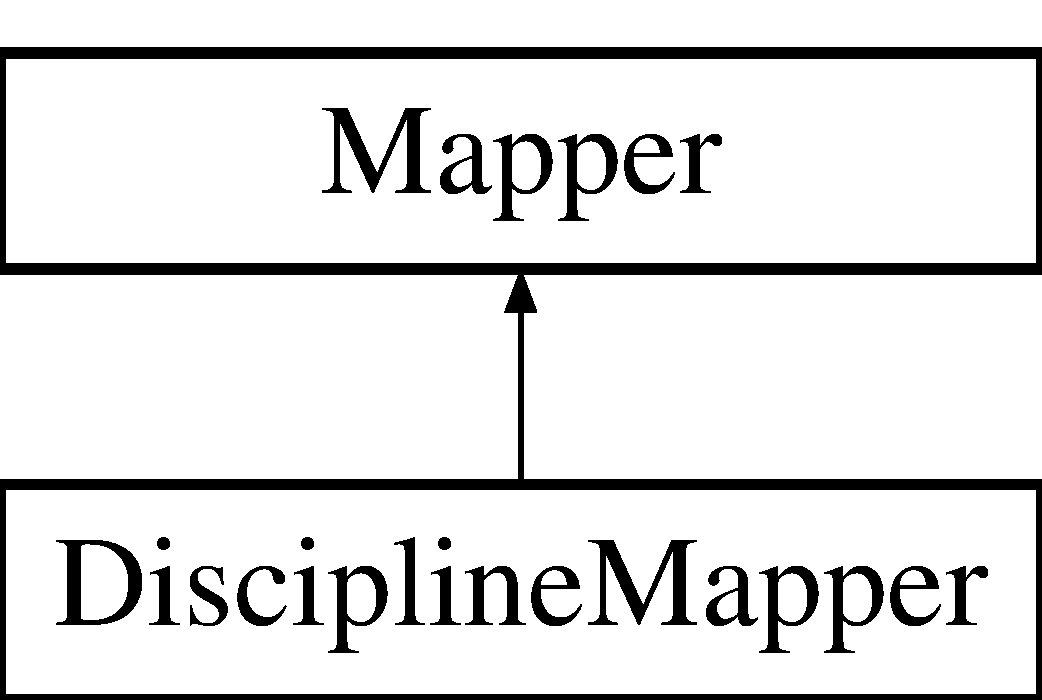
\includegraphics[height=2.000000cm]{classDisciplineMapper}
\end{center}
\end{figure}
\subsection*{Открытые члены}
\begin{DoxyCompactItemize}
\item 
\hypertarget{classDisciplineMapper_a7ec50024e3c9fbdbf843db27bceb2a7b}{}{\bfseries \+\_\+\+\_\+construct} (\$db)\label{classDisciplineMapper_a7ec50024e3c9fbdbf843db27bceb2a7b}

\item 
\hyperlink{classDisciplineMapper_a96fde87c7447aea528ee1982286c5bfb}{read} (array \$zapoc)
\end{DoxyCompactItemize}
\subsection*{Дополнительные унаследованные члены}


\subsection{Методы}
\hypertarget{classDisciplineMapper_a96fde87c7447aea528ee1982286c5bfb}{}\index{Discipline\+Mapper@{Discipline\+Mapper}!read@{read}}
\index{read@{read}!Discipline\+Mapper@{Discipline\+Mapper}}
\subsubsection[{read}]{\setlength{\rightskip}{0pt plus 5cm}Discipline\+Mapper\+::read (
\begin{DoxyParamCaption}
\item[{array}]{\$zapoc}
\end{DoxyParamCaption}
)}\label{classDisciplineMapper_a96fde87c7447aea528ee1982286c5bfb}
\begin{DoxyReturn}{Возвращает}
\hyperlink{classDisciplines}{Disciplines} a discipline table module object 
\end{DoxyReturn}


Объявления и описания членов класса находятся в файле\+:\begin{DoxyCompactItemize}
\item 
backend/student.\+php\end{DoxyCompactItemize}

\hypertarget{classDisciplines}{}\section{Класс Disciplines}
\label{classDisciplines}\index{Disciplines@{Disciplines}}
Граф наследования\+:Disciplines\+:\begin{figure}[H]
\begin{center}
\leavevmode
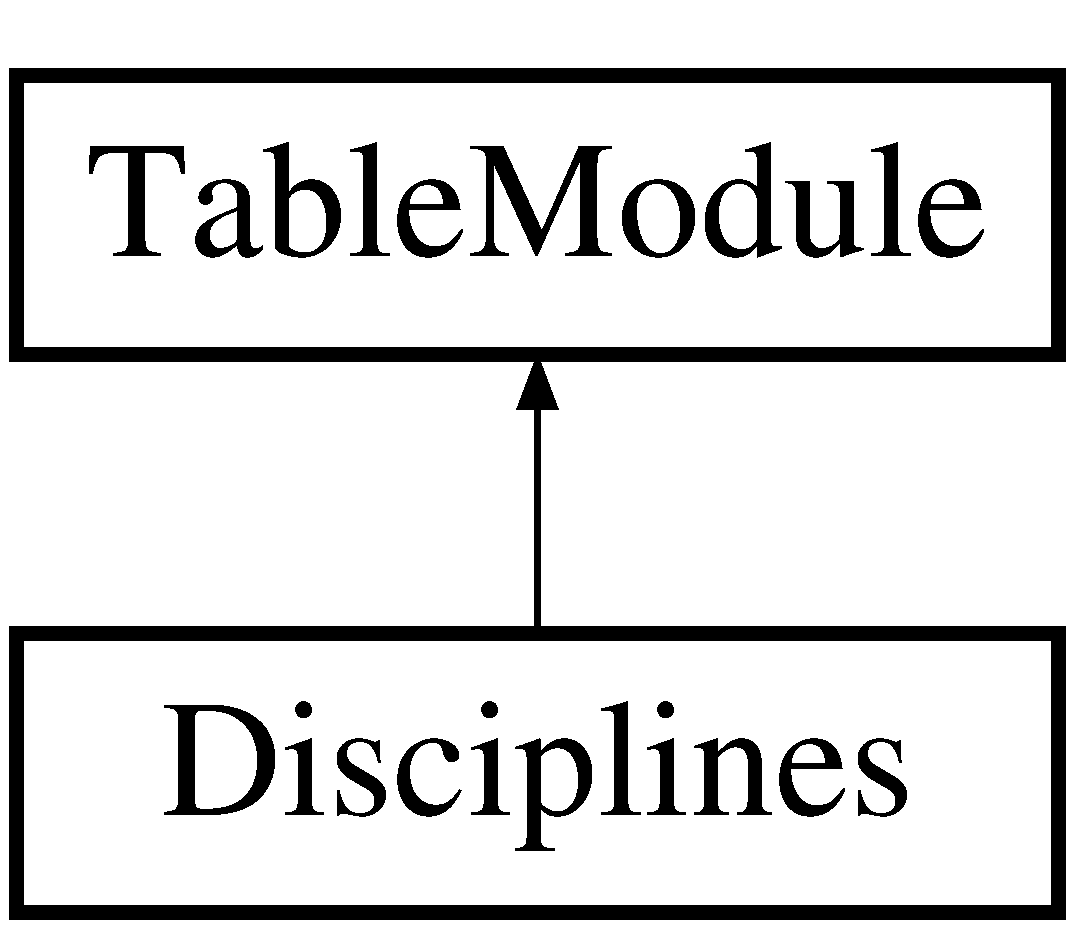
\includegraphics[height=2.000000cm]{classDisciplines}
\end{center}
\end{figure}
\subsection*{Открытые члены}
\begin{DoxyCompactItemize}
\item 
\hypertarget{classDisciplines_a68fc713c8f3709f5f41d7f64009f4f0b}{}{\bfseries view} ()\label{classDisciplines_a68fc713c8f3709f5f41d7f64009f4f0b}

\end{DoxyCompactItemize}
\subsection*{Дополнительные унаследованные члены}


Объявления и описания членов класса находятся в файле\+:\begin{DoxyCompactItemize}
\item 
backend/student.\+php\end{DoxyCompactItemize}

\hypertarget{classDisciplinesModel}{}\section{Класс Disciplines\+Model}
\label{classDisciplinesModel}\index{Disciplines\+Model@{Disciplines\+Model}}
Граф наследования\+:Disciplines\+Model\+:\begin{figure}[H]
\begin{center}
\leavevmode
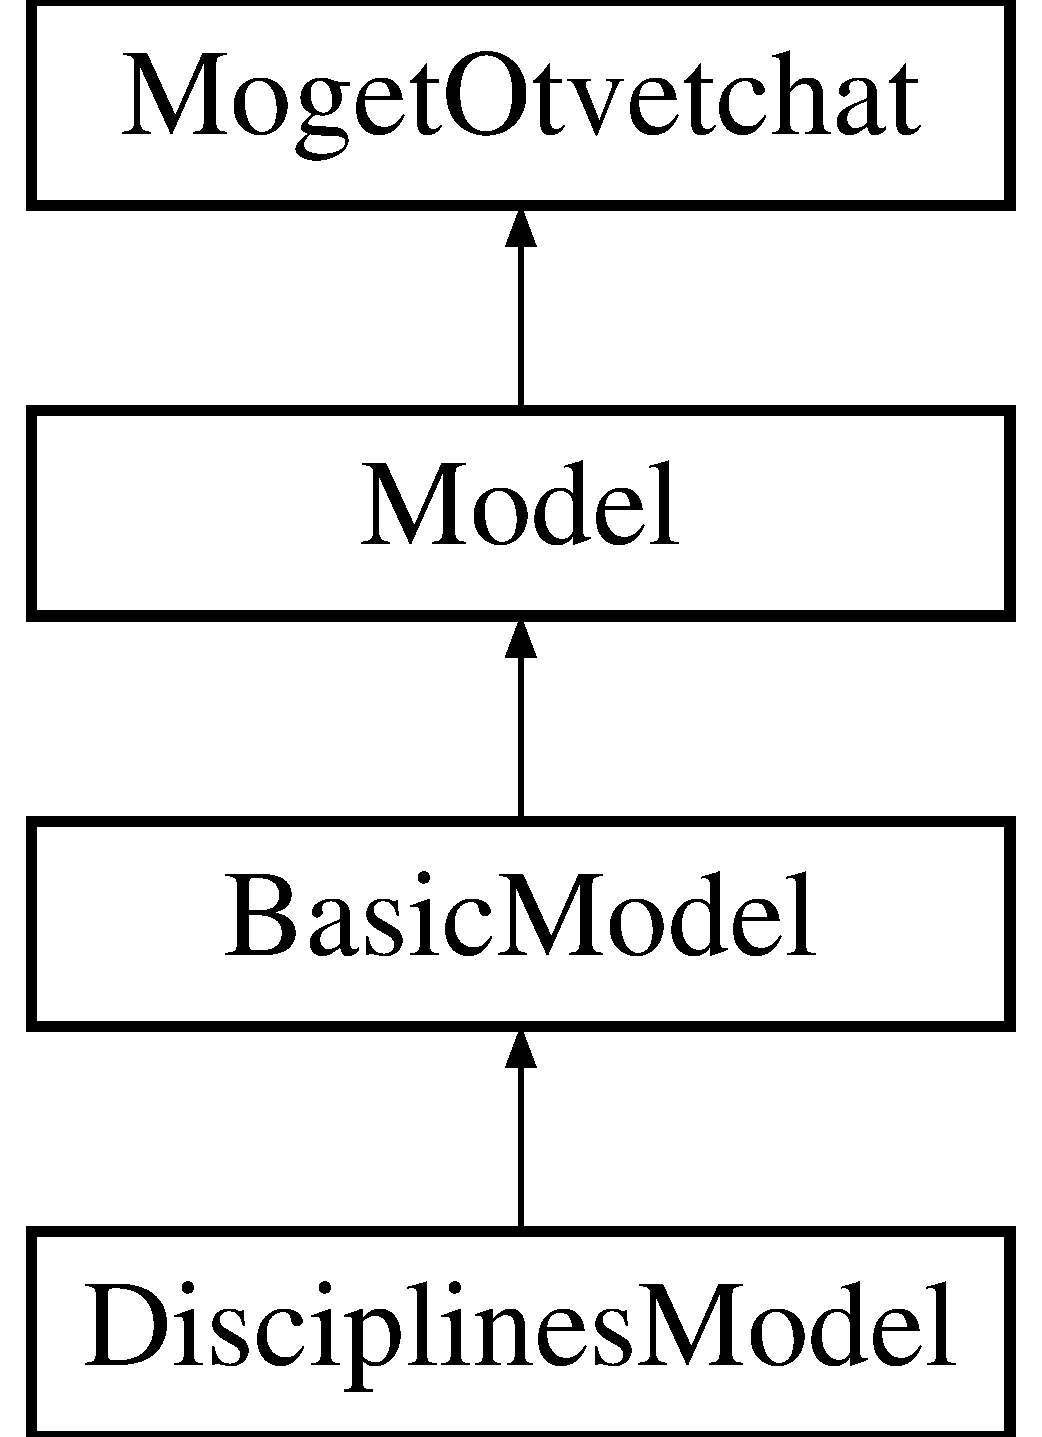
\includegraphics[height=4.000000cm]{classDisciplinesModel}
\end{center}
\end{figure}
\subsection*{Открытые члены}
\begin{DoxyCompactItemize}
\item 
\hypertarget{classDisciplinesModel_a7c8da1c7efc4bf05398ad5f53de5c26f}{}{\bfseries \+\_\+\+\_\+construct} (\$db)\label{classDisciplinesModel_a7c8da1c7efc4bf05398ad5f53de5c26f}

\end{DoxyCompactItemize}


Объявления и описания членов класса находятся в файле\+:\begin{DoxyCompactItemize}
\item 
backend/Disciplines\+Model.\+php\end{DoxyCompactItemize}

\hypertarget{classLayerCommunication}{}\section{Класс Layer\+Communication}
\label{classLayerCommunication}\index{Layer\+Communication@{Layer\+Communication}}
\subsection*{Открытые члены}
\begin{DoxyCompactItemize}
\item 
\hypertarget{classLayerCommunication_a53c655ae003463769c4f9010d0ff6f1f}{}{\bfseries \+\_\+\+\_\+construct} (\hyperlink{classDatabase}{Database} \$db, \$modules)\label{classLayerCommunication_a53c655ae003463769c4f9010d0ff6f1f}

\item 
\hypertarget{classLayerCommunication_a28f965d9e36a8f3997663d7ac81de816}{}{\bfseries otvetchat} (\$query)\label{classLayerCommunication_a28f965d9e36a8f3997663d7ac81de816}

\end{DoxyCompactItemize}


Объявления и описания членов класса находятся в файле\+:\begin{DoxyCompactItemize}
\item 
backend/Layer\+Communication.\+php\end{DoxyCompactItemize}

\hypertarget{classMapper}{}\section{Класс Mapper}
\label{classMapper}\index{Mapper@{Mapper}}
Граф наследования\+:Mapper\+:\begin{figure}[H]
\begin{center}
\leavevmode
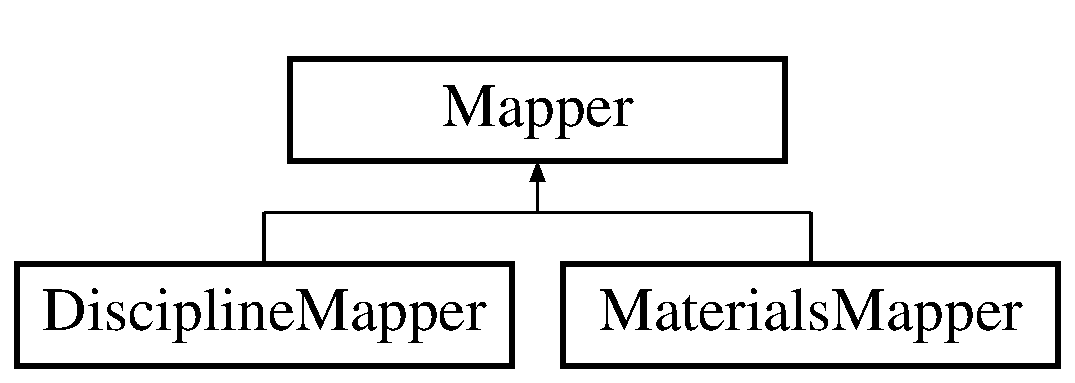
\includegraphics[height=2.000000cm]{classMapper}
\end{center}
\end{figure}
\subsection*{Открытые члены}
\begin{DoxyCompactItemize}
\item 
\hypertarget{classMapper_ac57073adb354fedfc5397e3ffb029cf1}{}{\bfseries \+\_\+\+\_\+construct} (\hyperlink{classDatabase}{Database} \$db, \$table)\label{classMapper_ac57073adb354fedfc5397e3ffb029cf1}

\item 
\hypertarget{classMapper_a3690aa0032657dfa1c22d6b40fa6c689}{}{\bfseries read} (array \$zaproc)\label{classMapper_a3690aa0032657dfa1c22d6b40fa6c689}

\end{DoxyCompactItemize}
\subsection*{Открытые статические члены}
\begin{DoxyCompactItemize}
\item 
\hypertarget{classMapper_a0d08e8a60d7614c31a3ab5891ed4f73f}{}static {\bfseries fabric} (\hyperlink{classDatabase}{Database} \$db, \$name)\label{classMapper_a0d08e8a60d7614c31a3ab5891ed4f73f}

\end{DoxyCompactItemize}
\subsection*{Защищенные члены}
\begin{DoxyCompactItemize}
\item 
\hypertarget{classMapper_a998edf9bcef41624c8a1ccc7de78bbaf}{}{\bfseries fill\+Model} (\$module)\label{classMapper_a998edf9bcef41624c8a1ccc7de78bbaf}

\end{DoxyCompactItemize}


Объявления и описания членов класса находятся в файле\+:\begin{DoxyCompactItemize}
\item 
backend/student.\+php\end{DoxyCompactItemize}

\hypertarget{classMaterials}{}\section{Класс Materials}
\label{classMaterials}\index{Materials@{Materials}}
Граф наследования\+:Materials\+:\begin{figure}[H]
\begin{center}
\leavevmode
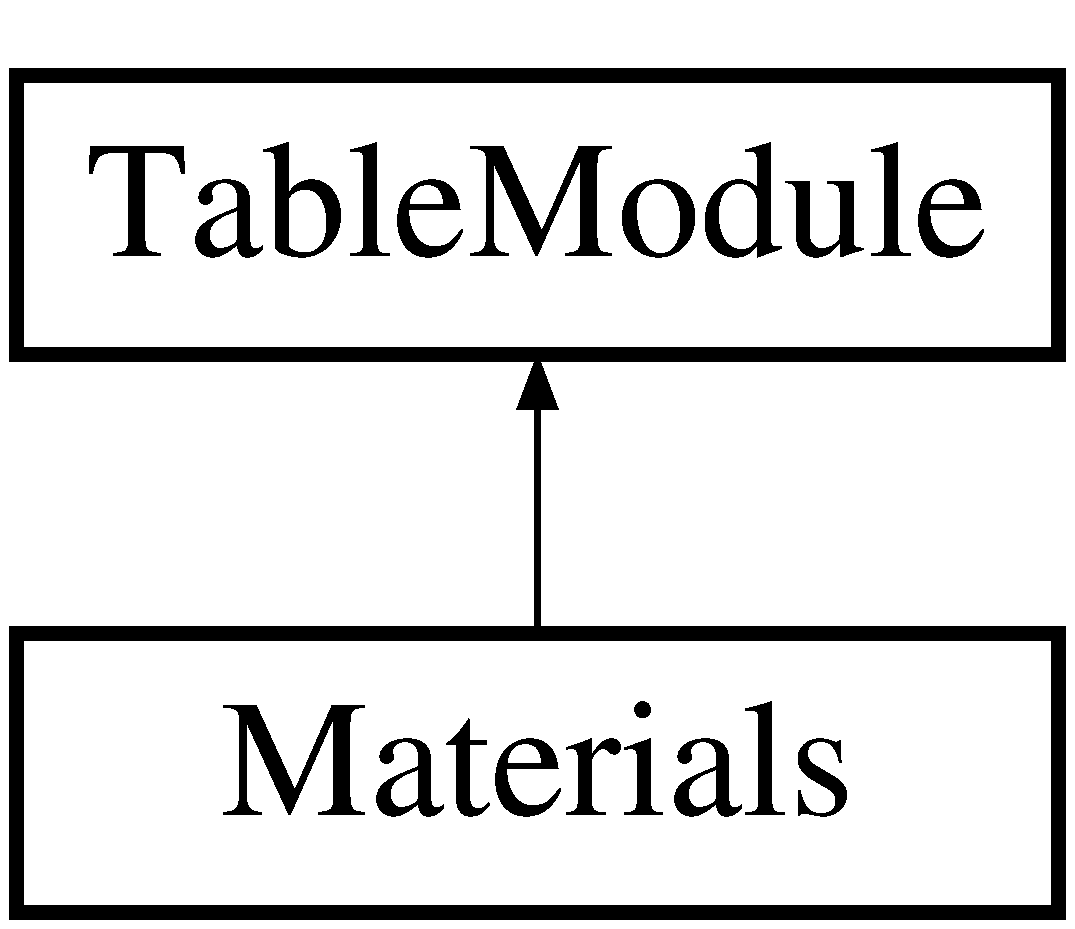
\includegraphics[height=2.000000cm]{classMaterials}
\end{center}
\end{figure}
\subsection*{Открытые члены}
\begin{DoxyCompactItemize}
\item 
\hypertarget{classMaterials_af3fb9f614af27713d7ea69ae5f64ba85}{}{\bfseries \+\_\+\+\_\+construct} (\$discipline, \$search)\label{classMaterials_af3fb9f614af27713d7ea69ae5f64ba85}

\item 
\hypertarget{classMaterials_a1ab137318da4a6c06cd5ae098a471906}{}{\bfseries view} ()\label{classMaterials_a1ab137318da4a6c06cd5ae098a471906}

\item 
\hypertarget{classMaterials_ac1d9d2cfe2a07432695703004c43e55b}{}{\bfseries add} (array \$row)\label{classMaterials_ac1d9d2cfe2a07432695703004c43e55b}

\end{DoxyCompactItemize}
\subsection*{Дополнительные унаследованные члены}


Объявления и описания членов класса находятся в файле\+:\begin{DoxyCompactItemize}
\item 
backend/student.\+php\end{DoxyCompactItemize}

\hypertarget{classMaterialsMapper}{}\section{Класс Materials\+Mapper}
\label{classMaterialsMapper}\index{Materials\+Mapper@{Materials\+Mapper}}
Граф наследования\+:Materials\+Mapper\+:\begin{figure}[H]
\begin{center}
\leavevmode
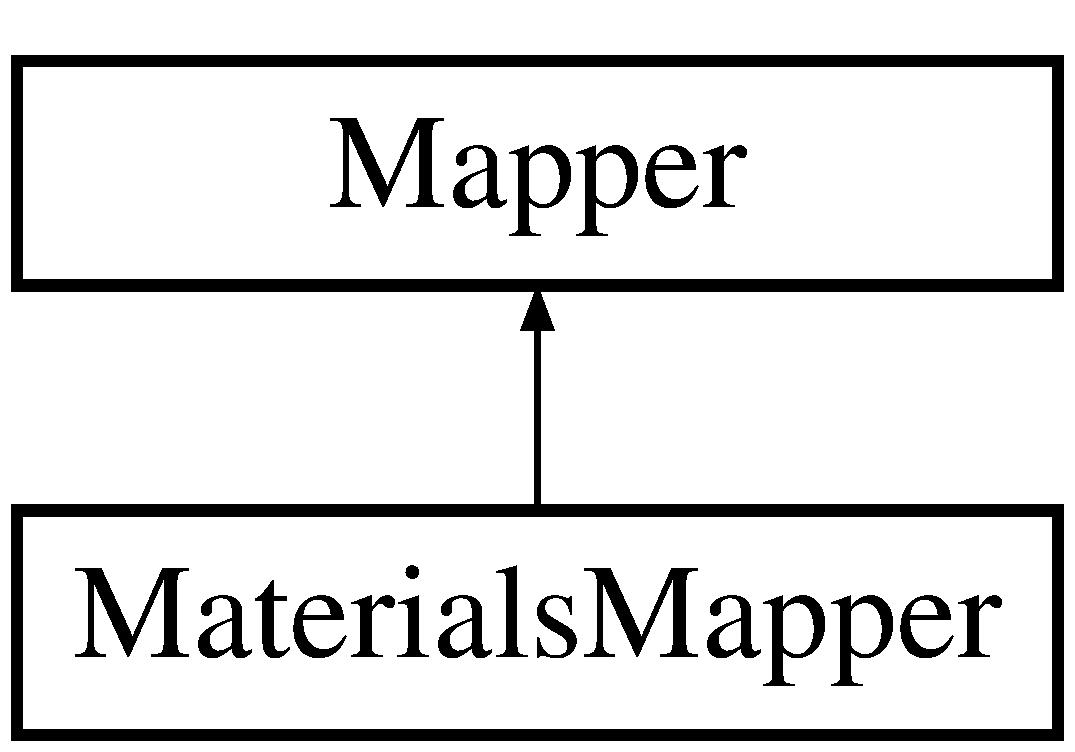
\includegraphics[height=2.000000cm]{classMaterialsMapper}
\end{center}
\end{figure}
\subsection*{Открытые члены}
\begin{DoxyCompactItemize}
\item 
\hypertarget{classMaterialsMapper_a8a554e9c2a71e53b0155667e07193690}{}{\bfseries \+\_\+\+\_\+construct} (\$db)\label{classMaterialsMapper_a8a554e9c2a71e53b0155667e07193690}

\item 
\hyperlink{classMaterialsMapper_adf49b44aa89ed1b363637ce0a60e1ff9}{read} (array \$zaproc)
\end{DoxyCompactItemize}
\subsection*{Дополнительные унаследованные члены}


\subsection{Методы}
\hypertarget{classMaterialsMapper_adf49b44aa89ed1b363637ce0a60e1ff9}{}\index{Materials\+Mapper@{Materials\+Mapper}!read@{read}}
\index{read@{read}!Materials\+Mapper@{Materials\+Mapper}}
\subsubsection[{read}]{\setlength{\rightskip}{0pt plus 5cm}Materials\+Mapper\+::read (
\begin{DoxyParamCaption}
\item[{array}]{\$zaproc}
\end{DoxyParamCaption}
)}\label{classMaterialsMapper_adf49b44aa89ed1b363637ce0a60e1ff9}
\begin{DoxyReturn}{Возвращает}
\hyperlink{classDisciplines}{Disciplines} \+: a discipline table module object 
\end{DoxyReturn}


Объявления и описания членов класса находятся в файле\+:\begin{DoxyCompactItemize}
\item 
backend/student.\+php\end{DoxyCompactItemize}

\hypertarget{classMaterialsModel}{}\section{Класс Materials\+Model}
\label{classMaterialsModel}\index{Materials\+Model@{Materials\+Model}}
Граф наследования\+:Materials\+Model\+:\begin{figure}[H]
\begin{center}
\leavevmode
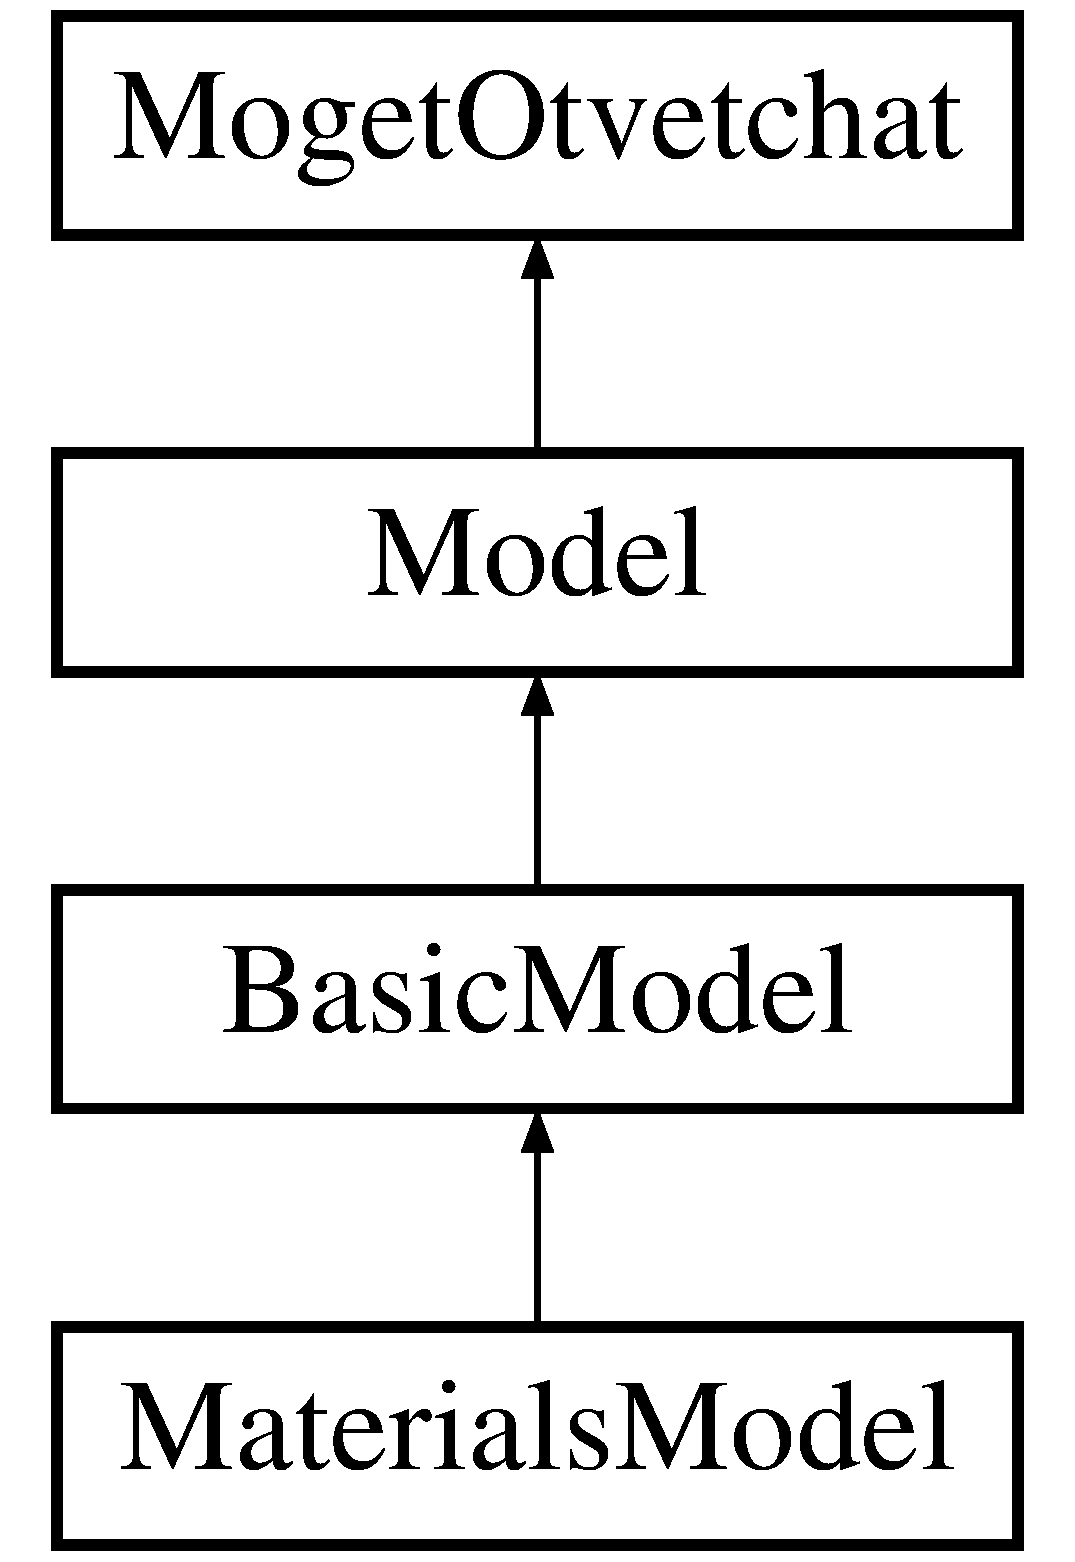
\includegraphics[height=4.000000cm]{classMaterialsModel}
\end{center}
\end{figure}
\subsection*{Открытые члены}
\begin{DoxyCompactItemize}
\item 
\hypertarget{classMaterialsModel_aafd370a9667837fee7b852f37af3425d}{}{\bfseries \+\_\+\+\_\+construct} (\$db)\label{classMaterialsModel_aafd370a9667837fee7b852f37af3425d}

\end{DoxyCompactItemize}


Объявления и описания членов класса находятся в файле\+:\begin{DoxyCompactItemize}
\item 
backend/Materials\+Model.\+php\end{DoxyCompactItemize}

\hypertarget{classModel}{}\section{Класс Model}
\label{classModel}\index{Model@{Model}}
Граф наследования\+:Model\+:\begin{figure}[H]
\begin{center}
\leavevmode
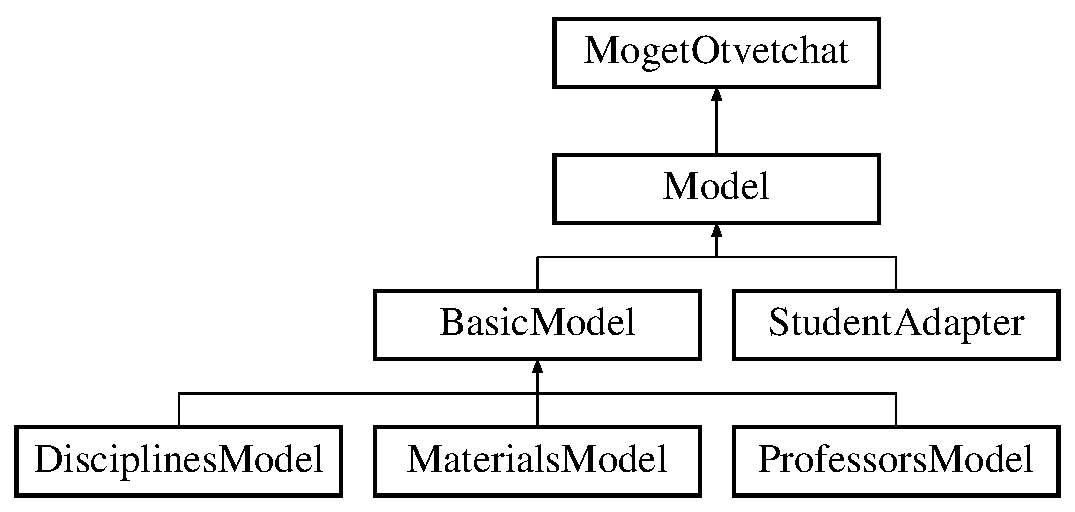
\includegraphics[height=4.000000cm]{classModel}
\end{center}
\end{figure}
\subsection*{Открытые члены}
\begin{DoxyCompactItemize}
\item 
\hyperlink{classModel_a63b113c5ec29c2295af8c097402f71f2}{otvetchat} (array \$zaproc)
\item 
\hypertarget{classModel_afb2431e9128d7e08adf8b1b71c33df01}{}{\bfseries get\+Value} (array \$zaproc)\label{classModel_afb2431e9128d7e08adf8b1b71c33df01}

\item 
\hyperlink{classModel_ac06d31e467a180c245c13a59fb6132f3}{set\+Next} (\hyperlink{interfaceMogetOtvetchat}{Moget\+Otvetchat} \$next)
\item 
\hypertarget{classModel_af63457f86c986fe181bd0501f90a9fde}{}{\bfseries get\+Next} ()\label{classModel_af63457f86c986fe181bd0501f90a9fde}

\item 
\hypertarget{classModel_a4f6f22d1c991579ccd4e56b09c20ef2b}{}{\bfseries set\+Name} (\$name)\label{classModel_a4f6f22d1c991579ccd4e56b09c20ef2b}

\item 
\hypertarget{classModel_a99ae6ab8071fc0d1e62894ce22edf5ad}{}{\bfseries get\+Name} ()\label{classModel_a99ae6ab8071fc0d1e62894ce22edf5ad}

\end{DoxyCompactItemize}


\subsection{Методы}
\hypertarget{classModel_a63b113c5ec29c2295af8c097402f71f2}{}\index{Model@{Model}!otvetchat@{otvetchat}}
\index{otvetchat@{otvetchat}!Model@{Model}}
\subsubsection[{otvetchat}]{\setlength{\rightskip}{0pt plus 5cm}Model\+::otvetchat (
\begin{DoxyParamCaption}
\item[{array}]{\$zaproc}
\end{DoxyParamCaption}
)}\label{classModel_a63b113c5ec29c2295af8c097402f71f2}
Answer the given query. If the current class cannot answer the query, it will be transmitted to the next one in the chain. 
\begin{DoxyParams}{Аргументы}
{\em query} & query parameters \\
\hline
\end{DoxyParams}
\begin{DoxyReturn}{Возвращает}
A character string that will be transmitted to the client 
\end{DoxyReturn}


Замещает \hyperlink{interfaceMogetOtvetchat_aee06b6431e3e3af9c73ff16ee9be5525}{Moget\+Otvetchat}.

\hypertarget{classModel_ac06d31e467a180c245c13a59fb6132f3}{}\index{Model@{Model}!set\+Next@{set\+Next}}
\index{set\+Next@{set\+Next}!Model@{Model}}
\subsubsection[{set\+Next}]{\setlength{\rightskip}{0pt plus 5cm}Model\+::set\+Next (
\begin{DoxyParamCaption}
\item[{{\bf Moget\+Otvetchat}}]{\$next}
\end{DoxyParamCaption}
)}\label{classModel_ac06d31e467a180c245c13a59fb6132f3}
Define the next element in the chain \begin{DoxyReturn}{Возвращает}
The object itself 
\end{DoxyReturn}


Замещает \hyperlink{interfaceMogetOtvetchat_a7e2c5b60d5f9ca86416f32fe00e356fb}{Moget\+Otvetchat}.



Объявления и описания членов класса находятся в файле\+:\begin{DoxyCompactItemize}
\item 
backend/Model.\+php\end{DoxyCompactItemize}

\hypertarget{interfaceMogetOtvetchat}{}\section{Интерфейс Moget\+Otvetchat}
\label{interfaceMogetOtvetchat}\index{Moget\+Otvetchat@{Moget\+Otvetchat}}
Граф наследования\+:Moget\+Otvetchat\+:\begin{figure}[H]
\begin{center}
\leavevmode
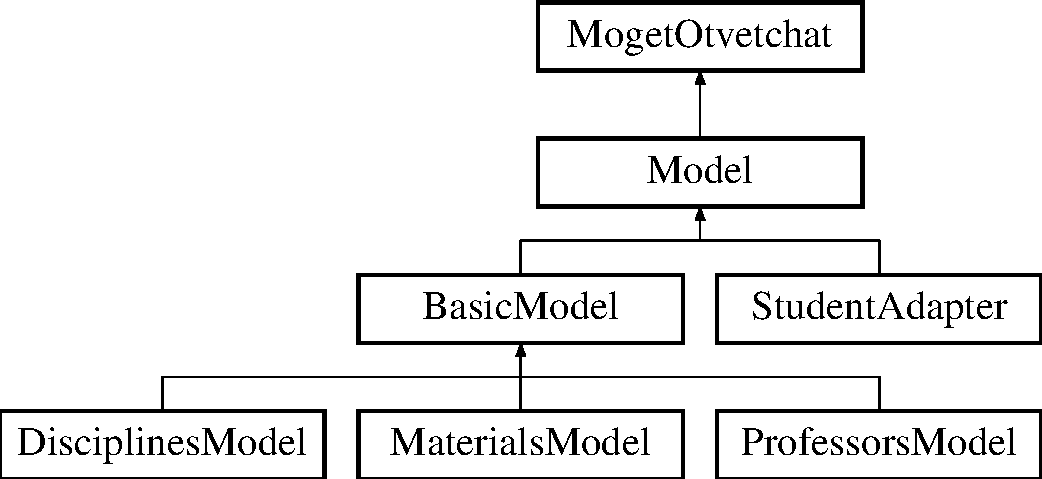
\includegraphics[height=4.000000cm]{interfaceMogetOtvetchat}
\end{center}
\end{figure}
\subsection*{Открытые члены}
\begin{DoxyCompactItemize}
\item 
\hyperlink{interfaceMogetOtvetchat_aee06b6431e3e3af9c73ff16ee9be5525}{otvetchat} (array \$zaproc)
\item 
\hyperlink{interfaceMogetOtvetchat_a7e2c5b60d5f9ca86416f32fe00e356fb}{set\+Next} (\hyperlink{interfaceMogetOtvetchat}{Moget\+Otvetchat} \$next)
\end{DoxyCompactItemize}


\subsection{Подробное описание}
Interface that modules entering the chain of responsability have to implement. Defines a class that can answer to an H\+T\+T\+P request. 

\subsection{Методы}
\hypertarget{interfaceMogetOtvetchat_aee06b6431e3e3af9c73ff16ee9be5525}{}\index{Moget\+Otvetchat@{Moget\+Otvetchat}!otvetchat@{otvetchat}}
\index{otvetchat@{otvetchat}!Moget\+Otvetchat@{Moget\+Otvetchat}}
\subsubsection[{otvetchat}]{\setlength{\rightskip}{0pt plus 5cm}Moget\+Otvetchat\+::otvetchat (
\begin{DoxyParamCaption}
\item[{array}]{\$zaproc}
\end{DoxyParamCaption}
)}\label{interfaceMogetOtvetchat_aee06b6431e3e3af9c73ff16ee9be5525}
Answer the given query. If the current class cannot answer the query, it will be transmitted to the next one in the chain. 
\begin{DoxyParams}{Аргументы}
{\em query} & query parameters \\
\hline
\end{DoxyParams}
\begin{DoxyReturn}{Возвращает}
A character string that will be transmitted to the client 
\end{DoxyReturn}


Замещается в \hyperlink{classStudentAdapter_a3bef77fa5ced3e0c7fa7f79cc958c41e}{Student\+Adapter} и \hyperlink{classModel_a63b113c5ec29c2295af8c097402f71f2}{Model}.

\hypertarget{interfaceMogetOtvetchat_a7e2c5b60d5f9ca86416f32fe00e356fb}{}\index{Moget\+Otvetchat@{Moget\+Otvetchat}!set\+Next@{set\+Next}}
\index{set\+Next@{set\+Next}!Moget\+Otvetchat@{Moget\+Otvetchat}}
\subsubsection[{set\+Next}]{\setlength{\rightskip}{0pt plus 5cm}Moget\+Otvetchat\+::set\+Next (
\begin{DoxyParamCaption}
\item[{{\bf Moget\+Otvetchat}}]{\$next}
\end{DoxyParamCaption}
)}\label{interfaceMogetOtvetchat_a7e2c5b60d5f9ca86416f32fe00e356fb}
Define the next element in the chain \begin{DoxyReturn}{Возвращает}
The object itself 
\end{DoxyReturn}


Замещается в \hyperlink{classModel_ac06d31e467a180c245c13a59fb6132f3}{Model}.



Объявления и описания членов интерфейса находятся в файле\+:\begin{DoxyCompactItemize}
\item 
backend/Moget\+Otvetchat.\+php\end{DoxyCompactItemize}

\hypertarget{classProfessorsModel}{}\section{Класс Professors\+Model}
\label{classProfessorsModel}\index{Professors\+Model@{Professors\+Model}}
Граф наследования\+:Professors\+Model\+:\begin{figure}[H]
\begin{center}
\leavevmode
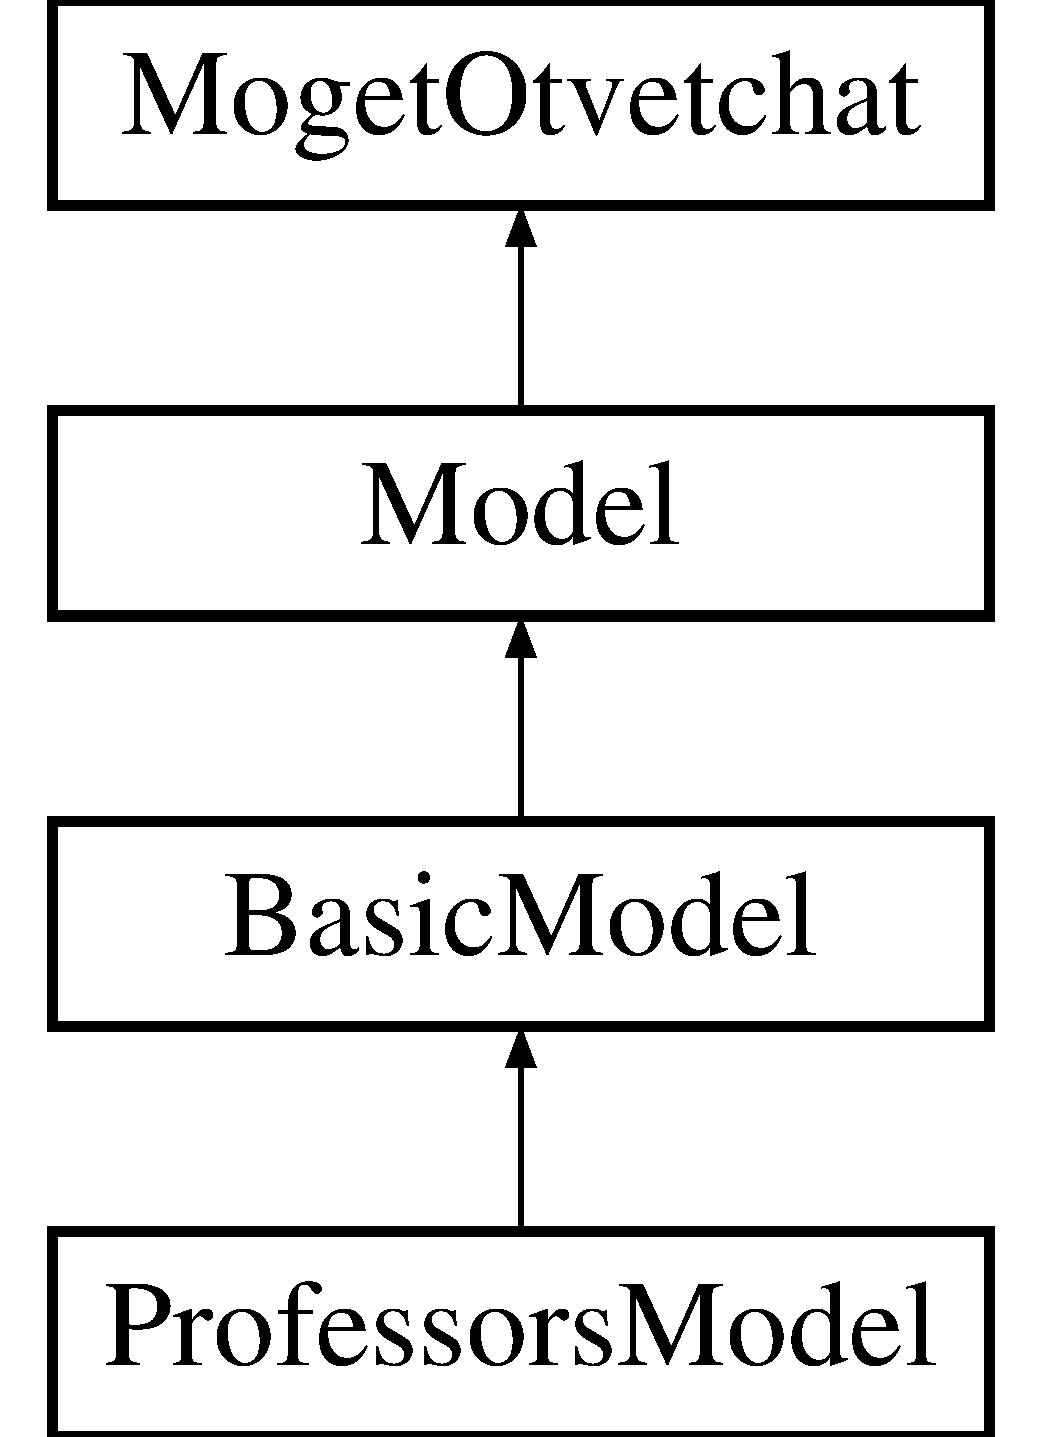
\includegraphics[height=4.000000cm]{classProfessorsModel}
\end{center}
\end{figure}
\subsection*{Открытые члены}
\begin{DoxyCompactItemize}
\item 
\hypertarget{classProfessorsModel_a9407334912449fea657c4df215748518}{}{\bfseries \+\_\+\+\_\+construct} (\$db)\label{classProfessorsModel_a9407334912449fea657c4df215748518}

\end{DoxyCompactItemize}


Объявления и описания членов класса находятся в файле\+:\begin{DoxyCompactItemize}
\item 
backend/Professors\+Model.\+php\end{DoxyCompactItemize}

\hypertarget{classStudentAdapter}{}\section{Класс Student\+Adapter}
\label{classStudentAdapter}\index{Student\+Adapter@{Student\+Adapter}}
Граф наследования\+:Student\+Adapter\+:\begin{figure}[H]
\begin{center}
\leavevmode
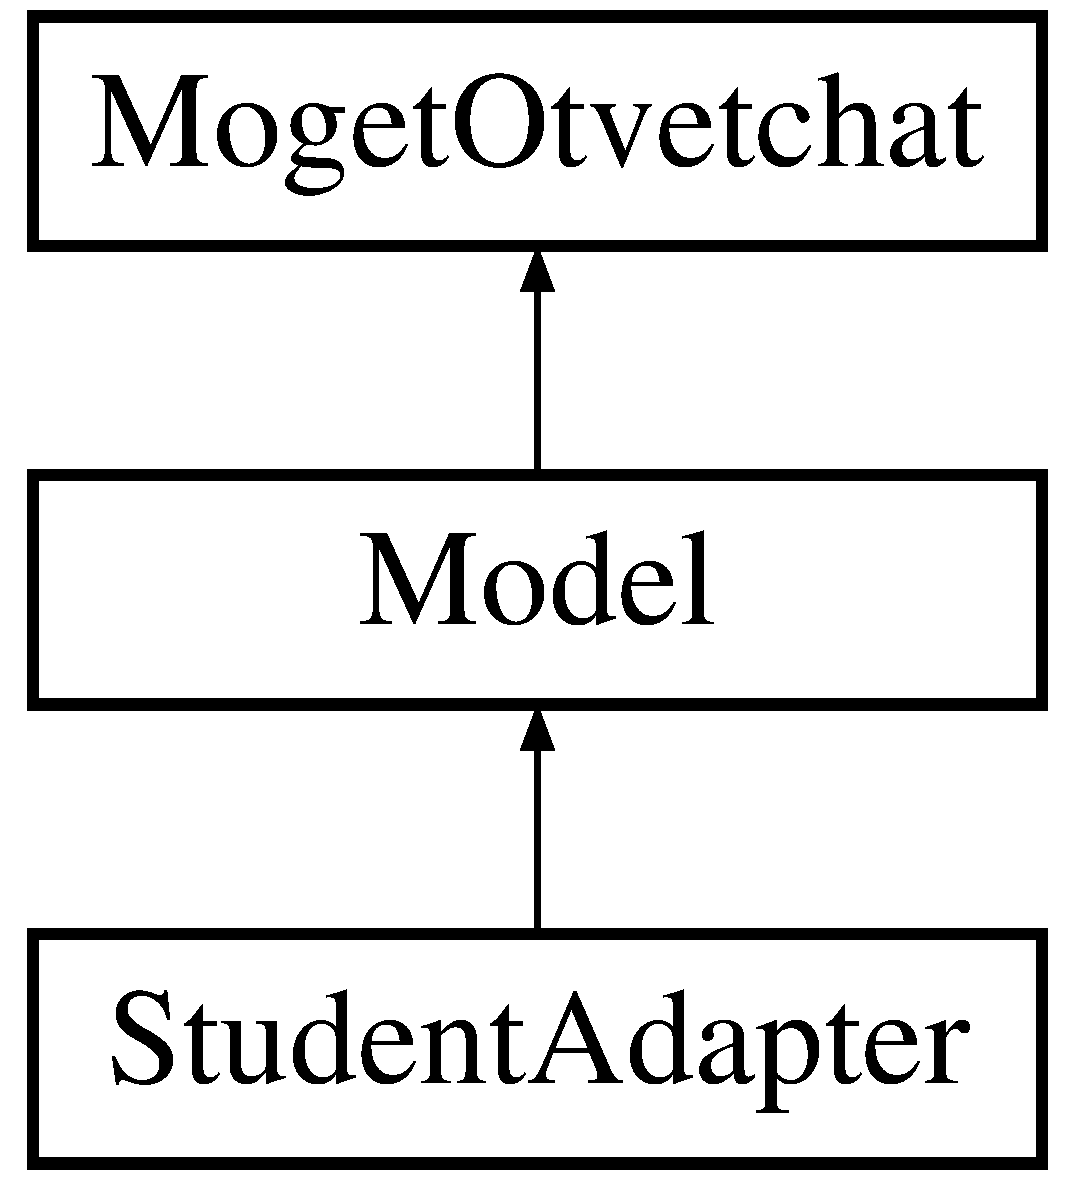
\includegraphics[height=3.000000cm]{classStudentAdapter}
\end{center}
\end{figure}
\subsection*{Открытые члены}
\begin{DoxyCompactItemize}
\item 
\hypertarget{classStudentAdapter_ae6560cbd781b9e517aa49c0e21094f06}{}{\bfseries \+\_\+\+\_\+construct} (\$name, \hyperlink{classMapper}{Mapper} \$mapper)\label{classStudentAdapter_ae6560cbd781b9e517aa49c0e21094f06}

\item 
\hyperlink{classStudentAdapter_a3bef77fa5ced3e0c7fa7f79cc958c41e}{otvetchat} (array \$zaproc)
\item 
\hypertarget{classStudentAdapter_a0fd80b842054b227cdd14f5fd368ef70}{}{\bfseries get\+Value} (array \$zaproc)\label{classStudentAdapter_a0fd80b842054b227cdd14f5fd368ef70}

\end{DoxyCompactItemize}
\subsection*{Открытые статические члены}
\begin{DoxyCompactItemize}
\item 
\hypertarget{classStudentAdapter_abe36356a6d7e1d90ecb6b084c59dd8a7}{}static {\bfseries fabric} (\hyperlink{classDatabase}{Database} \$db, \$name)\label{classStudentAdapter_abe36356a6d7e1d90ecb6b084c59dd8a7}

\end{DoxyCompactItemize}


\subsection{Методы}
\hypertarget{classStudentAdapter_a3bef77fa5ced3e0c7fa7f79cc958c41e}{}\index{Student\+Adapter@{Student\+Adapter}!otvetchat@{otvetchat}}
\index{otvetchat@{otvetchat}!Student\+Adapter@{Student\+Adapter}}
\subsubsection[{otvetchat}]{\setlength{\rightskip}{0pt plus 5cm}Student\+Adapter\+::otvetchat (
\begin{DoxyParamCaption}
\item[{array}]{\$zaproc}
\end{DoxyParamCaption}
)}\label{classStudentAdapter_a3bef77fa5ced3e0c7fa7f79cc958c41e}
Answer the given query. If the current class cannot answer the query, it will be transmitted to the next one in the chain. 
\begin{DoxyParams}{Аргументы}
{\em query} & query parameters \\
\hline
\end{DoxyParams}
\begin{DoxyReturn}{Возвращает}
A character string that will be transmitted to the client 
\end{DoxyReturn}


Замещает \hyperlink{interfaceMogetOtvetchat_aee06b6431e3e3af9c73ff16ee9be5525}{Moget\+Otvetchat}.



Объявления и описания членов класса находятся в файле\+:\begin{DoxyCompactItemize}
\item 
backend/student.\+php\end{DoxyCompactItemize}

\hypertarget{classTableModule}{}\section{Класс Table\+Module}
\label{classTableModule}\index{Table\+Module@{Table\+Module}}
Граф наследования\+:Table\+Module\+:\begin{figure}[H]
\begin{center}
\leavevmode
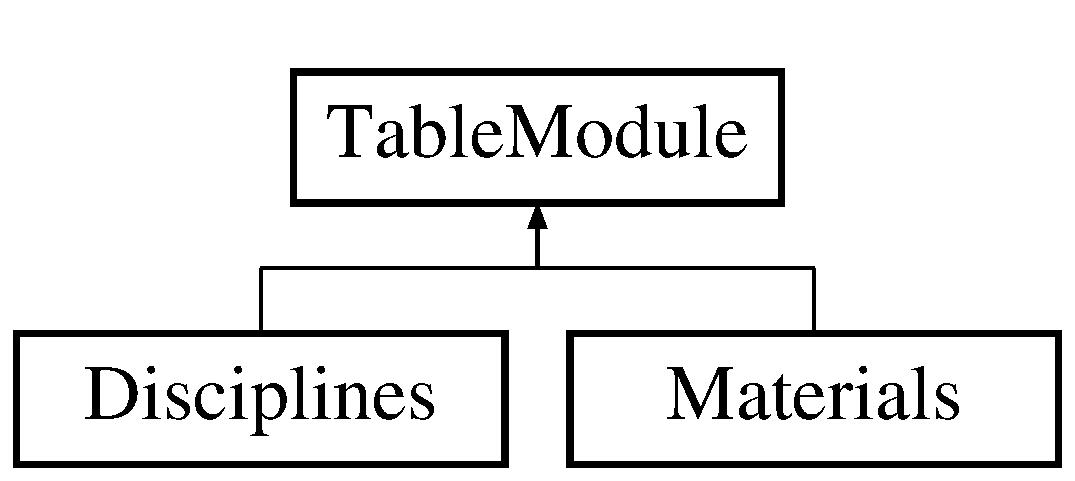
\includegraphics[height=2.000000cm]{classTableModule}
\end{center}
\end{figure}
\subsection*{Открытые члены}
\begin{DoxyCompactItemize}
\item 
\hypertarget{classTableModule_a27518974022238398e72de9a827848cd}{}{\bfseries add} (array \$row)\label{classTableModule_a27518974022238398e72de9a827848cd}

\item 
\hypertarget{classTableModule_accce62f4d1a5cb55b004552d62a610d0}{}{\bfseries view} ()\label{classTableModule_accce62f4d1a5cb55b004552d62a610d0}

\end{DoxyCompactItemize}
\subsection*{Защищенные члены}
\begin{DoxyCompactItemize}
\item 
\hypertarget{classTableModule_a751eb37cbca98bf3457ccfaa36b1416a}{}{\bfseries get\+Rows} ()\label{classTableModule_a751eb37cbca98bf3457ccfaa36b1416a}

\end{DoxyCompactItemize}


\subsection{Подробное описание}
Buisines Logic\+: table module pattern 

Объявления и описания членов класса находятся в файле\+:\begin{DoxyCompactItemize}
\item 
backend/student.\+php\end{DoxyCompactItemize}

%--- End generated contents ---

% Index
\backmatter
\newpage
\phantomsection
\clearemptydoublepage
\addcontentsline{toc}{chapter}{Алфавитный указатель}
\printindex

\end{document}
